\documentclass{article}
\usepackage[utf8]{inputenc}
\usepackage{amsmath}
\usepackage{framed}
\usepackage{titlesec}
\usepackage{shadethm}
\usepackage{xcolor}
\usepackage{minted}
\usepackage{graphicx}

\title{Error Plotting, Recursion, Newton-Raphson Iteration}
\author{MATH2072}
\date{\today}

\newcommand{\sectionbreak}{\clearpage}

\newshadetheorem{prototheorem}{Theorem}
\newenvironment{theorem}
	{\definecolor{shadethmcolor}{HTML}{EDF8FF}\definecolor{shaderulecolor}{HTML}{45CFFF}\setlength{\shadeboxrule}{.4pt}\begin{prototheorem}\normalfont}
	{\end{prototheorem}}
\newshadetheorem{protodefinition}{Definition}
\newenvironment{definition}
	{\definecolor{shadethmcolor}{HTML}{FFD6a1}\definecolor{shaderulecolor}{HTML}{FFA32B}\setlength{\shadeboxrule}{.4pt}\begin{protodefinition}\normalfont}
	{\end{protodefinition}}
\newshadetheorem{protocorollary}{Corollary}
\newenvironment{corollary}
	{\definecolor{shadethmcolor}{HTML}{D4FFEB}\definecolor{shaderulecolor}{HTML}{21FF97}\setlength{\shadeboxrule}{.4pt}\begin{protocorollary}\normalfont}
	{\end{protocorollary}}
\newshadetheorem{protoremark}{Remark}
\newenvironment{remark}
	{\definecolor{shadethmcolor}{HTML}{DFD4FF}\definecolor{shaderulecolor}{HTML}{713DFF}\setlength{\shadeboxrule}{.4pt}\begin{protoremark}\normalfont}
	{\end{protoremark}}
\newshadetheorem{protoexample}{Example}
\newenvironment{example}
	{\definecolor{shadethmcolor}{HTML}{FFB0B0}\definecolor{shaderulecolor}{HTML}{FF3D3D}\setlength{\shadeboxrule}{.4pt}\begin{protoexample}\normalfont}
	{\end{protoexample}}

\begin{document}
\part*{Lecture 4\\Error Plotting, Recursion, Newton-Raphson Iteration}

\section*{Summary of Last Lecture}

\subsection*{Bisection}
\begin{itemize}
	\item Evaluate function only.
	\item Need to find $a$ and $b$ such that $f$ is continuous and has unique zero on $[a,b]$. 
	\item Upper bound for error: $|x^{(k)} \leq \epsilon^{(k)} = |b^{(k)}-a^{(k)}|$.
	\item Decreases as $\epsilon^{(k+1)}=\frac{\epsilon^{(k)}}{2}$...
	\item ...so that $\epsilon^{(k)}=\frac{\epsilon^{(0)}}{2^k}$, aka \textit{linear} convergence. 
	\item Straight line on semilog plot.
	\item Works only for one unknown. Adobe
\end{itemize}

\subsection*{Newton's Method/Secant Method}
\begin{itemize}
	\item Uses function and derivative/two initial points.
	\item Function must be continuously differentiable/continuous around $x^*$.
	\item Need one/two initial guesses.
	\item Error estimate: $\epsilon^{(k+1)} \approx |\delta x^{(k)}|$.
	\item Decreases as $\epsilon^{(k+1)} \approx (\epsilon^{(k)})^{2^k}$...
	\item ... so that $\epsilon^{(k)} \approx (\epsilon^{(0)})^{2^k}$, aka \textit{quadratic} convergence.
	\item Steeper than linear on semilog plot.  
\end{itemize}

\clearpage

\section*{Error Plotting of Newton's vs. Secant Method}

\begin{figure*}
	\centering
	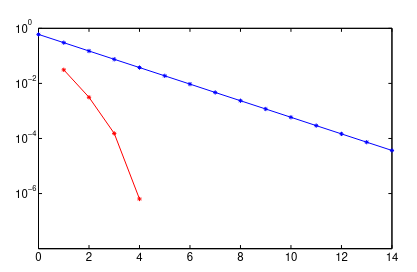
\includegraphics[width=\textwidth]{res/04a.png}
	\caption{}
\end{figure*}
\clearpage

\section*{Recursion}

Simple example of recursive programming:

\begin{minted}{python}
def bisection(a, b, k_max, eps_x, eps_f):
	mid = (a + b) / 2
	x = mid
	err = abs(a - b) / 2\]
	fm = func(mid)
	res = abs(fmid)
	if k_max > 0:
		if err > eps_x or res > eps_f:
			fa = func(a)
			if fm * fa > 0:
				a = mid
			else:
				b = mid
			x, err, res = bisection(a, b, k_max - 1, eps_x, eps_f)
	else:
		print("Warning: no convergence...")
	return x, err, res
\end{minted}

\textbf{Pros:}
\begin{itemize}
	\item clean, concise, elegant code;
	\item conceptually clear.
\end{itemize}

\textbf{Cons:}
\begin{itemize}
	\item code harder to follow;
	\item uses more memory;
	\item small mistake can give bad crash! 
\end{itemize}

\section*{Newton-Raphson Iteration}
\begin{remark}
Newton iteration can be generalized to $n$ equations with $n$ unknowns. 

Alternative derivation in 1D:
\[
f(x+\delta x)\approx f(x) + f'(x)\delta x = 0\implies\delta x = -\frac{f(x)}{f'(x)}
\]

Now in 2D. We want to find $x_1$ and $x_2$ such that: 
\[
f_1(x_1, x_2)=0
\]\[
f_2(x_1, x_2)=0
\]

Note that in general, we need \textbf{the same number of equations and unknowns} to find (isolated) solutions.
\[
f_1(x_1 + \delta x_1, x_2 + \delta x_2) \approx f_1(x_1, x_2) + \frac{\partial f_1}{\partial x_1}(x_1, x_2)\delta x_1 + \frac{\partial f_1}{\partial x_2}(x_1, x_2)\delta x_2
\]\[
f_2(x_1+\delta x_1, x_2+\delta x_2)\approx f_1(x_1,x_2)+\frac{\partial f_2}{\partial x_1}(x_1,x_2)\delta x_1 + \frac{\partial f_2}{\partial x_2}(x_1, x_2)\delta x_2
\]

which gives:
\[
\begin{bmatrix}
\frac{\partial f_1}{\partial x_1}(x_1, x_2) & \frac{\partial f_1}{\partial x_2}(x_1, x_2) \\
\frac{\partial f_2}{\partial x_1}(x_1, x_2) & \frac{\partial f_2}{\partial x_2}(x_1, x_2) 
\end{bmatrix}
\begin{bmatrix}
\delta x_1 \\
\delta x_2
\end{bmatrix}
=-
\begin{bmatrix}
f_1(x_1, x_2) \\
f_2(x_1, x_2) 
\end{bmatrix}
\]
\end{remark}
\end{document}